\chapter{Projektverlauf und Meilensteine} \label{ch:projektverlauf}
\section{Programmentwurf und Architekturentwurf}
\todo{rewrite}

Der Entwurf des Programms sowie die Architektur von CYBRAIL basieren auf einer klaren Strukturierung der Funktionalitäten, um eine effiziente und erweiterbare Lösung zu gewährleisten. 
Im folgenden Abschnitt wird der Architekturentwurf näher erläutert, gefolgt von einem detaillierten Blick auf die wichtigsten Klassen und deren Interaktionen.

\subsection{Architekturentwurf}

Das Architekturdiagramm (siehe Abbildung \ref{fig
}) zeigt die modulare Struktur des Systems. 
CYBRAIL ist in verschiedene Schichten unterteilt, um die Verantwortlichkeiten klar voneinander zu trennen und eine flexible Erweiterbarkeit zu ermöglichen. Die wichtigsten Schichten sind:

\begin{itemize} 
\item \textbf{Benutzeroberfläche (UI):} Diese Schicht stellt die Interaktion mit den Anwendern sicher und bietet eine intuitive Oberfläche, um Prüfungen und Auswertungen zu verwalten. 
Sie ermöglicht die Anzeige von Logdaten, Konfigurationsmöglichkeiten und die Ausgabe der Analyseergebnisse. 
\item \textbf{Analyse-Engine:} Das Herzstück von CYBRAIL ist die Analyse-Engine, die die gesammelten Logdaten nach Auffälligkeiten untersucht. 
Diese Schicht enthält alle notwendigen Algorithmen, um potenzielle Betrugsversuche zu erkennen und entsprechende Berichte zu generieren. 
\item \textbf{Datenverwaltung:} Hier werden alle eingehenden Daten verarbeitet und in geeigneten Datenbanken gespeichert. 
Diese Schicht sorgt für den Zugriff auf Logdateien, Konfigurationsdaten und andere notwendige Informationen. 
\item \textbf{Schnittstellen zur Datenquelle:} Die unterste Schicht stellt die Anbindung an externe Systeme wie den Safe Exam Browser (\gls{seb}) sicher. 
Hier werden Logdaten gesammelt und über definierte Schnittstellen an die Datenverwaltung und Analyse-Engine weitergeleitet. \end{itemize}

\begin{landscape}
\begin{figure}[h]
    \centering
    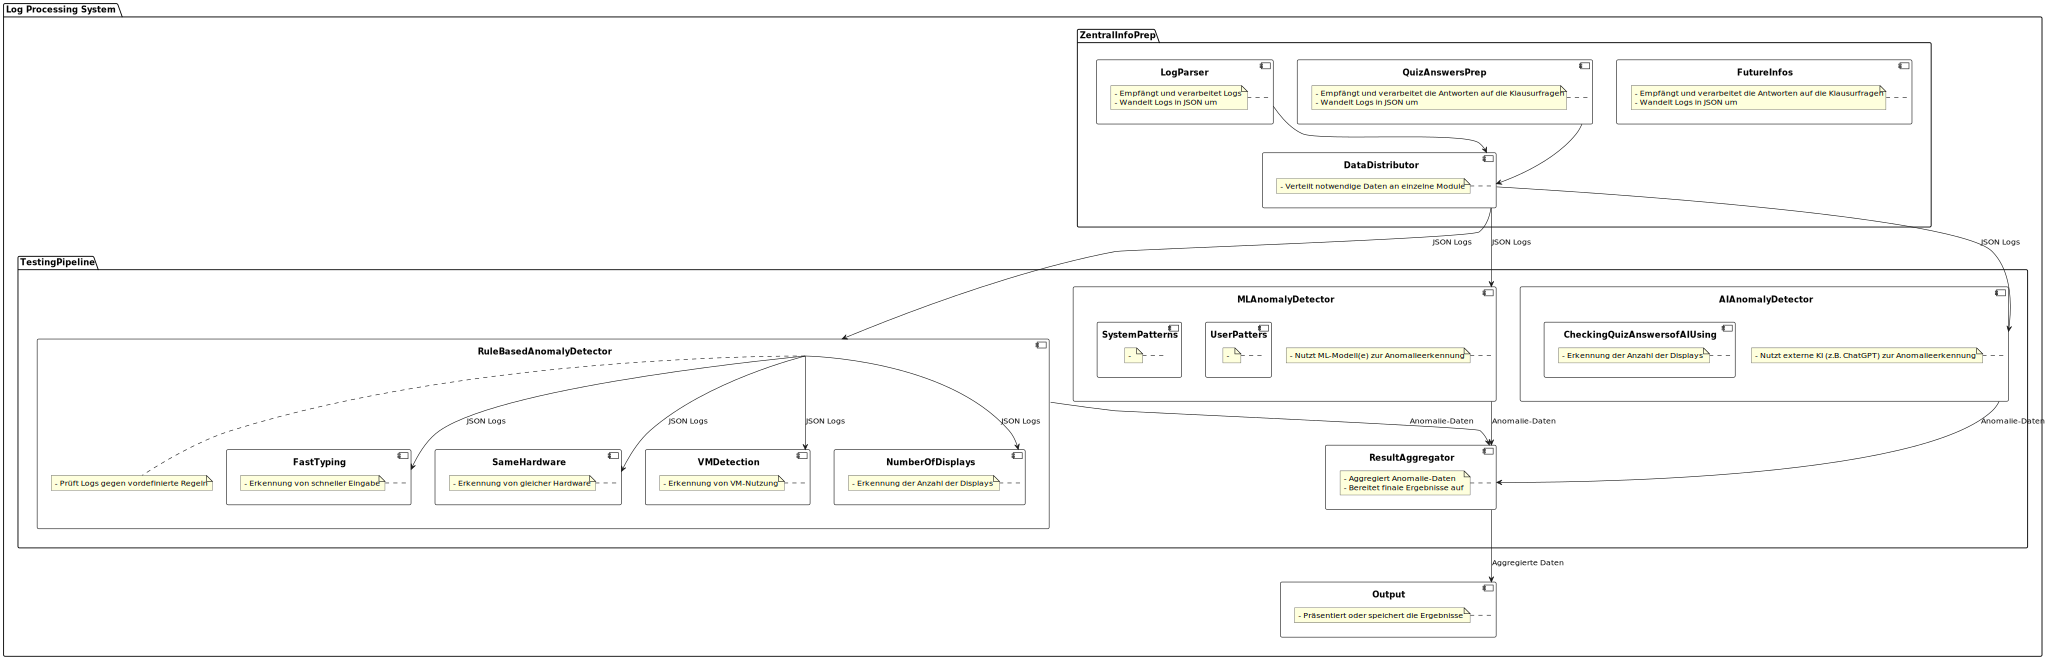
\includegraphics[width=1.5\textwidth]{figures/CybrailArchitektur.pdf}
    \caption{Klassendiagramm von CYBRAIL}
        \label{fig:klassendiagramm}
\end{figure}
\end{landscape}

Durch diese modulare Architektur ist es möglich, einzelne Komponenten unabhängig voneinander zu entwickeln, zu testen und bei Bedarf auszutauschen, ohne das Gesamtsystem zu beeinträchtigen.

\subsection{Programmentwurf}

Das Klassendiagramm in Abbildung \ref{fig
} verdeutlicht die wichtigsten Klassen und deren Beziehungen innerhalb des Systems. 
Die zentrale Klasse ist \texttt{LogAnalyzer}, welche für die Analyse der Logdaten zuständig ist. 
Die wichtigsten Klassen und deren Funktionen sind:

\begin{itemize} 
\item \texttt{LogAnalyzer}: Diese Klasse enthält die Logik zur Auswertung der Logdateien und identifiziert potenzielles Fehlverhalten basierend auf vorgegebenen Regeln und Mustern. 
\item \texttt{LogFile}: Stellt eine Abstraktion für eine Logdatei dar.
Diese Klasse übernimmt das Einlesen und Vorverarbeiten der Logs, die dann vom \texttt{LogAnalyzer} ausgewertet werden. 
\item \texttt{User}: Repräsentiert die Informationen zu einem Prüfling oder Nutzer des Systems. 
Diese Klasse wird insbesondere verwendet, um spezifische Daten während einer Prüfung zu speichern. 
\item \texttt{ReportGenerator}: Diese Klasse erstellt Berichte basierend auf den Ergebnissen der Loganalyse und bietet eine übersichtliche Darstellung der detektierten Auffälligkeiten. 
\end{itemize}

\begin{landscape}
\begin{figure}[h]
    \centering
    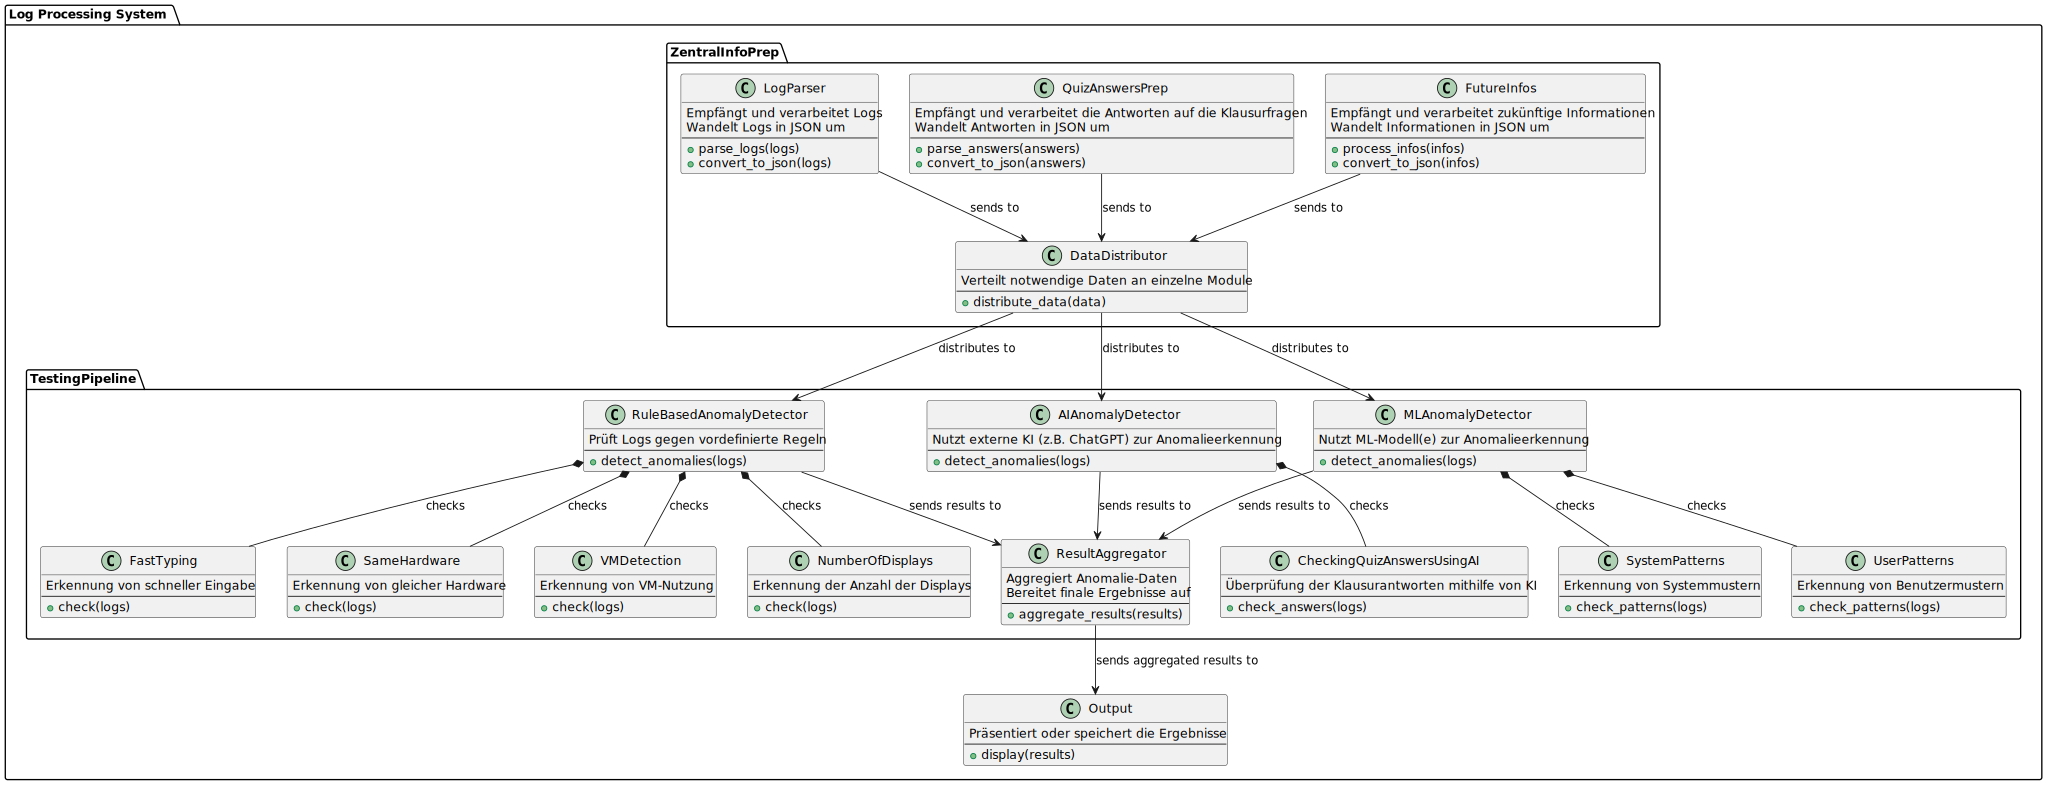
\includegraphics[width=1.5\textwidth]{figures/CybrailClassdiagramm.pdf}
    \caption{Architekturdiagramm von CYBRAIL}
    \label{fig:architekturdiagramm}
\end{figure}
\end{landscape}

Das Zusammenspiel dieser Klassen ermöglicht es, Logdaten effizient zu verarbeiten, Auffälligkeiten zu erkennen und verständliche Berichte für Prüfungsaufsichten zu generieren. 
Die modulare Struktur erlaubt es zudem, neue Regeln und Methoden zur Betrugserkennung hinzuzufügen, ohne bestehende Funktionalitäten zu beeinträchtigen.

\subsection{Zusammenfassung}

Der Architektur- und Programmentwurf von CYBRAIL folgt einem modularen Ansatz, der eine einfache Erweiterbarkeit und Wartbarkeit des Systems ermöglicht. Durch die klare Trennung der Verantwortlichkeiten kann CYBRAIL sowohl für die Verarbeitung großer Datenmengen als auch für eine schnelle Analyse in Echtzeit verwendet werden. Die klare Definition der Klassen und deren Aufgabenbereiche stellt sicher, dass das System flexibel auf neue Anforderungen angepasst werden kann.
